%\documentclass[10pt, conference, compsocconf]{IEEEtran}
%tire' de /home/ROCQ/aosteroc/fndoye/Documents/latex/icess2013/icess2013.tex

\documentclass[conference,compsocconf]{IEEEtran}
%\documentclass[11pt,twocolumn]{article}

\usepackage{algorithm}
\usepackage{algorithmic}
\usepackage[english]{babel}
\usepackage{verbatim}
\usepackage{amsmath} % assumes amsmath package installed
\usepackage{amsfonts}
\usepackage{epsfig,graphicx}
\usepackage{comment} 


\newcommand{\ds}{\displaystyle}
\newtheorem{proof}{proof}
\newtheorem{theorem}{Theorem}
\newtheorem{definition}{Definition}
\newtheorem{property}{Property}

\begin{document}

\title{Time Triggered Offline Scheduler for Data Dependent Real-Time Tasks
  Accounting for Preemption and Scheduler Costs}

%in ou for Time Critical Embedded Systems}

%\begin{comment}
\author{
\IEEEauthorblockN{Walid Talaboulma}
\IEEEauthorblockA{INRIA Paris-Rocquencourt\\
 Domaine de Voluceau BP 105\\
78153 Le Chesnay Cedex - France\\
walid.talaboulma@inria.fr}
\and    
\IEEEauthorblockN{Falou Ndoye}
\IEEEauthorblockA{INRIA Paris-Rocquencourt\\
 Domaine de Voluceau BP 105 \\
78153 Le Chesnay Cedex - France\\
falou.ndoye@inria.fr}
\and    
\IEEEauthorblockN{Yves Sorel }
\IEEEauthorblockA{INRIA Paris-Rocquencourt\\
 Domaine de Voluceau BP 105\\
78153 Le Chesnay Cedex - France\\
yves.sorel@inria.fr}
}
%\end{comment}
%\author{Sorel}

%\tableofcontents

\maketitle

\begin{abstract} Time critical embedded systems usually consist of a set of
  periodic data dependent real-time tasks which exchange data. Although
  non-preemptive real-time scheduling is safer than preemptive real-time
  scheduling in a time critical context, preemptive real-time scheduling
  provides a better success ratio. However, the preemption has a cost that it
  is risky to take into account imprecisely. In this paper we propose a
  schedulability analysis for data dependent periodic tasks which precisely
  accounts for preemption and scheduler costs. It results in a scheduling table
  that is exploited in a time triggered offline scheduler. We show that this
  scheduler, implemented on an ARM Cortex-M4 bare metal processor,
%requires very few memory and 
  is able to schedule correctly set of tasks that miss their deadline when
  preemption and scheduler costs are neglected. Therefore, such a scheduler is
  perfectly suited for time critical embedded systems.
\end{abstract}

%\begin{comment}
\begin{IEEEkeywords}
  \textit{time critical embedded systems, real-time scheduling, data dependent
    tasks, preemption cost, scheduler cost, offline schedulability analysis,
    time triggered scheduler, ARM Cortex-M4.}
\end{IEEEkeywords}
%\end{comment}

\section{Introduction}

We address time critical embedded systems, i.e. systems for which time
constraints must necessarily be satisfied in order to avoid catastrophic
consequences. Such systems, in most cases, consist of a set of data dependent
periodic tasks resulting from a functional specification, usually achieved with
tools such as Simulink \cite{simulink}, Scade \cite{scade}, etc., based on
block diagrams. The functional specification describes the functions that must
be executed, as well as their dependences carrying the data produced and
consumed by the functions. Such dependences involve a precedence relation on
the execution of every producer function relatively to one or several consumer
functions, and lead to sharing the transfered data. Data dependent functions
associated with temporal characteristics become data dependent real-time
tasks. Some of these characteristics like first releases, periods and deadlines
are not related to the processor that will execute the real-time tasks, whereas
the values of WCET (Worst Case Execution Time) depend on the processor.  Usual
schedulability analyses of periodic data dependent tasks are based on the WCET,
and thus, such analyses require that the designer determines accurately the
WCET which is strongly related to the internal architecture of the
processor. More this architecture is complex more it is difficult to determine
the WCET.

Although non-preemptive real-time scheduling is safer than preemptive real-time
scheduling in a time critical context, preemptive real-time scheduling provides
a better success ratio. However, the preemption has a cost that it is risky to
take into account imprecisely. The usual way to account for this cost, consists
in adding to the WCET of every task an extra cost which is a percentage of this
WCET. This approach may lead to miss some deadlines during the runtime
execution of the tasks even though the schedulability conditions have been
satisfied or, in the best case, resources could be wasted when this percentage
is chosen to high.

Therefore, on the one hand in order to guarantee the real-time schedulability
of a set of periodic data dependent tasks specifying a critical embedded
systems and on the other hand to minimize its needed resources, we propose a
schedulability analysis which takes into account precisely the cost of
preemption by counting them along a study interval. This analysis produces a
scheduling table that is exploited in a time triggered offline scheduler. We
give the principles of this scheduler and
%we achieve some simulations upon a Linux and a
%linux/Xenomai operating systems to validate the principles. Finally, 
implement it on an ARM Cortex-M4 bare metal processor. Then, whe show that this
implementation is able to schedule correctly a set of tasks that are not
correctly scheduled when preemption and scheduler costs are neglected.

The remainder of the paper is organized as follows. Section II presents the
related work on periodic data dependent tasks and on the preemption cost.
Section III presents the schedulability analysis. Section IV gives the
principles of the time triggered offline scheduler. Section V presents a
performance evaluation of the proposed scheduler on an ARM Cortex-M 4 bare
metal processor. Finally, Section VI concludes and gives some directions for
future work.

\section{Related Work}
\label{relWor}
We assume that the processor where the tasks will be executed, has neither
cache nor complex pipeline or specific internal architecture features. The
previous assumptions are usually made in time critical embedded systems where
determinism is a key issue. In this case, the preemption cost corresponds to
the duration necessary to save the context of the preempted task and the
duration necessary to restore this context when the preempted task will be
selected again to resume its execution. Due to its cost, a preemption increases
the response time of the preempted task that may cause another preemption, and
so on. The cost of the preemption is usually approximated in the WCET as
assumed, explicitly, by Liu and Layland in their pioneering article
\cite{LiuLayland73}. That is, some percentage of the WCET which corresponds to
the longest path in the sequential program associated to a task, is added to
its actual value. When the preemption cost is neglected, meaning this
percentage is close to zero, although a set of tasks verifies the
schedulability condition associated to the scheduling algorithm - which will be
implemented in the real-time scheduler -, some deadline misses may occur. In
order to tackle this problem, a first solution consists in determining the
maximum number of preemptions as proposed in \cite{BurnsTindellWellings95} or
in determining the number of preemptions but without accounting for the cost of
each preemption that can cause other preemptions, increasing the global cost in
\cite{EchagueRipollCrespo95}.  Other solutions aim at controlling the number of
preemptions, like presented in \cite{buttazzoBertogna13}. It is worth noting
that the preemption cost is not the only cost that must be precisely accounted
when dealing with time critical systems. 
%although it is easier to determine that the preemption cost,
Indeed, the scheduler cost itself must be also precisely accounted. Taking into
account the maximum number of preemptions and the scheduler cost, lead to
increase the WCET up to 50\%, for example in the most critical applications of
the avionic industry. This pessimism decreases the schedulability ratio and
increases the amount of necessary resources. On the other hand, a solution that
determines the exact number of preemptions while accounting for the cost of
each preemption is proposed in \cite{ecrts07}.  Unfortunately, this solution
assumes that the scheduling algorithm is based on fixed priorities.

Periodic data dependent tasks mean there are precedence constraints between
tasks \cite{Chetto90} such that a producer task is executed before the
corresponding consumer task, and the consumer task must receive the data
produced by the producer task. There are two approaches to dealing with
precedence constraints. The first one is based on semaphores \cite{forget11}. A
semaphore is allocated to each precedence, and the consumer task must wait for
the producer task to release the semaphore before it can start its
execution. The second approach is based on the modification of the priorities
and the release times of the task \cite{Chetto90,forget10}. Actually, when
dependent tasks have different periods the problem is much more complex than
when they have the same period \cite{richardCottetRichard01}. If the producer
task ${\tau_p}$ has a period smaller than the consumer task ${\tau_c}$, then
the latter has to consume in the worst case $n= \lfloor \frac {\tau_c}{\tau_p}
\rfloor$ data produced by the producer task. This worst case approach was
chosen in \cite{pdcs07}. Usually, only the last data is consumed since it is
considered to be the ``freshest'' one, like in
\cite{richardCottetRichard01}. Conversely, when the producer task has a period
greater than the consumer task, the latter has to consume at worst $n$ times
the same data produced by the producer task. Thus, it is sufficient that the
consumer task consumes only one of these data. When tasks are data dependent
they have to share some buffer containing the data that may involve priority
inversions. For example, a lower priority producer task can block the execution
of a consumer task that want to read it while it has a higher priority. In
order to avoid this situation the well known priority inheritance protocol that
gives to a task the highest priority of all the tasks which share a data, was
proposed in \cite{ShaRajkumarLehoczky90}.  This protocol holds only for static
priority scheduling algorithms. It was extended in \cite{ShaRajkumarLehoczky90}
by giving an additional priority to every shared data equal to the highest
priority of the tasks that share this data. This priority ceiling protocol
minimizes the blocking time and prevents deadlocks that may occur when several
tasks are mutually waiting for a shared data used by other tasks. For dynamic
priority scheduling algorithms, the stack resource policy was proposed in
\cite{baker91}.

In order to take into account precisely preemption and scheduler costs, an
offline schedulability analysis that considers the cost of each preemption, is
proposed in \cite{icse13}. Moreover, this analysis allows changes in the
priorities of the tasks that are necessary for dependent tasks which involve
priority inversions. In this paper after summarizing the principles of this
schedulability analysis, we show how it is exploited to implement an offline
scheduler executed at runtime that
%requires very few memory and 
is deterministic and thus perfectly suited for time critical embedded systems.

%voir ou mettre par la suite la phrase suivante : In our case the cost of the
%scheduler is reduced to a simple action that can be deterministically and
%precisely determined.

\section{Schedulability Analysis}

The schedulability analysis is based on a schedulability interval. This is a
finite time interval such that the schedule on this interval can be repeated
infinitely. We use the minimal schedulability interval for a set of $n$
periodic data dependent tasks proposed in \cite{ChoquetGrolleau04}. $I_n$
denotes the schedulability interval, given by:

\begin{equation}\label{int}
I_n=[r_{min},t_c+H_n] 
\end{equation}

where $t_c$ denotes the time from which the schedule repeats
indefinitely. $t_c$ is computed iteratively by an algorithm given in the
article. Since $t_c$ is smaller or equal to $r_{max}+H_n$,
%Afterwards, we assume that one of these schedulability intervals has been
%chosen to analyse $\Gamma_n$.
we will use thereafter the interval given by the Equation \ref{int} with
$tc=r_{max}+H_n$, $r_{min}$ and $r_{max}$ are respectively the minimum and the
maximum of the first release times $r_i^1$ of the tasks $\tau_i$ which is
released at times $r_i^k$, i.e. every instance (job) $k = 1..\infty$ of the
task.

$\Gamma_n$ denotes the set of periodic dependent tasks. The schedulability
analysis of $\Gamma_n$ is achieved on the schedulability interval $I_n$
according to a given fixed or dynamic priority scheduling algorithm, for
example Rate Monotonic (RM) or Earliest Deadline First (EDF)
\cite{LiuLayland73}, to cite only the most famous ones. Moreover, the release
times and the deadlines of every task are modified such that a task $\tau_j$
can be executed if and only if each of its predecessors $\tau_i$ produces
$k_{ij}=\lceil \frac{T_j}{T_i} \rceil$ data, and $\tau_j$ does not produce no
more than $k_{jk}=\lceil \frac{T_k}{T_j} \rceil$ data for each of its
successors $\tau_k$. These conditions guarantee that all the data produced are
consumed when two dependent tasks have equal or different periods and prevent
deadlocks between tasks. However, these conditions do not prevent priority
inversions due to the data shared by the dependent tasks. This is the reason
why we use, in the given scheduling algorithm, the priority inheritance
protocol \cite{ShaRajkumarLehoczky90} which minimizes the duration of priority
inversions.

The schedulability analysis performs a simulation of an offline scheduler that
is called only at release and completion times of every task. For every of
theses calls, denoted $t$, the schedulability analysis selects among the ready
tasks, with the function denoted $\phi:I(t) \to \Gamma_r(t) $, the task to
execute denoted $\tau_i$. Then, it computes the remaining execution time of
$\tau_i$ denoted $c_i:I(t) \to \mathbb{N}$ and the relative deadline of
$\tau_i$ denoted $d_i:I(t) \to \mathbb{N}$. These three functions are used to
test the schedulability of the task $\tau_i$. Finally, it determines the next
scheduler call. At the end of the schedulability interval $I_n$, if $\forall
\tau_i \in \Gamma_n$, $\tau_i$ is schedulable then $\Gamma_n$ is schedulable
and a scheduling table is produced, else $\Gamma_n$ is not schedulable.

\subsection{Task Selection $\phi(t)$}

When the scheduler is called at $t$, the task to be selected must belong to the
ready set of tasks denoted $\Gamma_r(t)$. A task $\tau_i$ is ready at $t$ if an
only if: its first release time occurs before, or at $t$, and it received all
the data produced by its predecessors, and all its successors consumed all the
data it produced. The selected task, denoted $\phi(t)$, is the task with the
highest priority in $\Gamma_r(t)$ according to the given scheduling algorithm
and the priority inheritance protocol.

\subsection{Remaining Execution Time $c_i(t)$}
\label{remExecTime}
$c_i(t)$ is the number of time units that $\tau_i$ must still execute at $t$ to
complete its execution. If $\tau_i$ is preempted at $t$, the cost of one
preemption is added to the remaining execution time $c_i(t)$ of $\tau_i$.

At every release or completion time of a task $\tau_i$ its remaining execution
time $c_i(t)$ is given by:

\begin{equation*}
       c_i(t)= \left\{
            \begin{array}{ll}
C_i   \ \ \ \ \ \ \ \ \ \ \ \ \ \ \ \ \ \ \  \ \ \ \ \ \ \  \ \mbox{if
  $(\frac{t-r_i^1}{T_i}) \in \mathbb{N} \ $  else} \\ 
\\
             c_i(r^{-}(t))   \ \ \ \ \ \ \ \ \ \ \ \ \ \ \ \ \ \ \
             \mbox{if $(\phi(r^{-}(t)) \neq \tau_i) \ $ else} \\ 
\\
           c_i(r^{-}(t))-(t-r^{-}(t)) \ \ \mbox{if $(\phi(t)=\tau_i) \vee $ }\\
%YS091214 supprime' 12 premiers "\" car "else" n'apparait pas
%     \mbox{$\ \ \ \ \ \  \ \ \ \ \ \ \ \ \  \ \ \ \ \ \ \ \ \  \ \ \ \ \ \  ((\phi(t) \neq \tau_i) \wedge (r^{-}(t)+c_i(r^{-}(t))= t))  \ \  $ else}\\

\mbox{$\ \ \ \; \ \ \ \ \   \ \ \ \ \ \ \ \  \ \ \ \ \ \ \ \
   \  \ \ \ \ \ \  ((\phi(t) \neq \tau_i) \wedge$}\\

%\mbox{$ ((\phi(t) \neq \tau_i) \wedge$}\\ 

 \mbox{$ \ \ \ \ \ \ \ \ \ \ \ \ \ \ \ \ \ \ \ \ \ \ (r^{-}(t)+c_i(r^{-}(t))= t))
   \ $ else}\\  
 \\

             c_i(r^{-}(t))-(t-r^{-}(t))+\alpha \ \ \  \mbox{} 
            \end{array}
          \right.
\end{equation*}

where $C_i$ denotes the WCET of $\tau_i$, $\alpha$ the cost of one preemption,
and $r^{-}(t)$ the previous scheduler call. It is important to note that the
WCET is considered here without any approximation of the preemption cost since
this cost is precisely taken into account with $\alpha$. However, the WCET
includes the precise cost for storing the context when a task is released while
preempting another task. In addition, it includes the precise cost of the
scheduler, as mentioned in the section \ref{relWor}, which is very simple in
our case and can be deterministically and precisely determined. This cost
consists in reading, in the scheduling table, the next task to execute when it
is released, or when it is resumed if this task were preempted. This is the
cost of the interruption routine given in section \ref{rts} where we present
the runtime scheduler algorithm \ref{algoSchedAna}.

In this computation there are four cases: 1) this is $\tau_i$ which is released
at $t$ and thus $c_i(t)=C_i$, 2) during the previous scheduler call the
selected task was different from $\tau_i$ and thus the remaining execution time
of $\tau_i$ does not change $c_i(t)=c_i(r^{-}(t))$, 3) during the previous
scheduler call the selected task was $\tau_i$ and it is not preempted at $t$,
meaning that $\tau_i$ is still the selected task at $t$ or, that $\tau_i$
completes its execution, thus $c_i(t)=c_i(r^{-}(t))-(t-r^{-}(t))$. That is, the
time elapsing between $t$ and the previous value of $t$ corresponding to the
execution time of $\tau_i$, is subtracted to the previous value of $c_i$, 4)
during the previous scheduler call the selected task was $\tau_i$ and $\tau_i$
is preempted at $t$, it follows that the cost of one preemption $\alpha$ is
added to $c_i(r^{-}(t))-(t-r^{-}(t))$.

Of course, this approach accounts for the cost of each preemption that can lead
to produce other preemptions.

The figure \ref{figRet} shows an example with two periodic tasks
$\tau_1(2,2,6,6)$ and $\tau_2(0,3,8,8)$ where the timing characteristics
between brackets correspond respectively to the first release time, the WCET,
the deadline, and the period. We assume that the scheduling algorithm is RM. In
this example, the offline scheduler is called at $t$ equal $0$, $2$, $4$, etc.,
corresponding to the release and completion times of both tasks $\tau_1$ and
$\tau_2$. At $t=0$, $\tau_2$ is released, thus $c_2(0)=3$. Then, at $t=2$,
$\tau_1$ is released, thus $c_1(2)=2$ and $\tau_2$ is preempted by $\tau_1$. A
time unit (in black) is added to take into account for the cost for restoring
the context of $\tau_2$ while the cost for storing the context of $\tau_2$ is
assumed to be included in the WCET of $\tau_1$, thus $c_2(2)=(3-2+0)+1=2$. For
the sake of simplicity, in this example we chose one time unit for the cost for
restoring the context, but actually it is widely smaller than the WCET. For the
same reason we do not show the cost for storing the context in the WCET of the
preempting task. See section \ref{costPreemp} to have an idea of the realistic
values of these costs.  At $t=4$, $\tau_1$ completes its execution, thus
$c_1(4)=2-4+2=0$ and $\tau_2$ resumes. Since during the previous scheduler call
$\tau_1$ was selected, which is different of $\tau_2$, thus $c_2(4)=c_2(2)=2$,
and so one for the other scheduler calls.

%It is worth noting that the latter cost (context restore) may be added several
%times according to the number of preemptions that the task suffers, whereas the
%former cost (contexte storage) is taken into account only one time for a given
%release (instance) of the task. By the way, this is the reason why we include
%this cost in the WCET of the preempting task. 

\begin{figure}[!h]
\begin{center}
\input{./images/cou-preemption_ci_sout.pspdftex}
\caption{Remaining execution time accounting for preemption cost}
%%%%%%%%%%%%%%%%%%%%%%%%%%%%%%%%%%%%%%%%%%%%%%%%%%%%%%%%%%%%%%%%%%%%%%%%%%%%
%YS voir avec Walid si on ajoute ici le cout du scheduler
% and scheduler costs} est-ce que l'algo l'ajoute au cout de store ds la tache
% qui preempte, sachant que l'autre partie est ds la tache preemptee
% alpha=sched+store+restore ?
\label{figRet}
\end{center}
\end{figure}

\subsection{Relative Deadline $d_i(t)$} 

At every release of $\tau_i$, $d_i(t)=D_i$, then $(t-r^{-}(t))$ is substracted
to $d_i(t)$ every time the scheduler is called. In order to do not miss its
deadline $\tau_i$ must complete its execution before date $t+d_i(t)$.

$d_i(t)$ is given by:

\begin{equation*}
  d_i(t)= \left\{
            \begin{array}{ll}
             D_i \ \ \ \ \ \ \ \ \ \ \ \ \ \ \ \ \ \ \ \ \ \ \ \ \ \ \mbox{if $(\frac{t-r_i^1}{T_i}) \in \mathbb{N} \ \ $ else } \\ \\
             d_i(r^{-}(t))-(t-r^{-}(t))  \mbox{\ if $r^{-}(t)+d_i(r^{-}(t))>t $}
               \\ \ \ \ \ \ \ \ \ \ \ \ \ \ \ \ \ \ \ \ \ \ \ \ \ \ \ \ \ \ \ \ \ \ \ \ \ \ \ \ \ \ \ \ \ \ \ \ \ \ \ \ \ \ else  \\ \\
             0 \ \ \  \mbox{} 
            \end{array}
          \right.
\end{equation*}

In this computation there are three cases: 1) the task $\tau_i$ is released at
$t$, 2) the previous scheduler call added to the previous relative deadline is
greater than the present scheduler call, thus the time elapsing between $t$ and
the previous value of $t$, is substracted to the previous value of $d_i$, 3)
the task $\tau_i$ completes or has already completed.

The figure \ref{figRd} shows an example with one task $\tau_i(0,3,8,8)$. At
$t=0$ the task $\tau_i$ is released, for the first time, thus $d_i(0)=8$. At
$t=2$, $r^{-}(2)-d_i(r^{-}(2))=0+8 > 2$, thus its relative deadline
$d_i(2)=8-2+0=6$ since its previous value was $d_i(0)=8$.

\begin{figure}[!h]
\begin{center}
\input{./images/di_t_sout.pspdftex}
\caption{Relative deadline}
\label{figRd}
\end{center}
\end{figure}

\subsection{Schedulability Condition at $t$}

The schedulability condition guarantees that the set of tasks is schedulable at
every scheduler call $t$. According to the theorem given in \cite{icse13}, a
task $\tau_i \in \Gamma_n$ is schedulable at $t$ if and only if:

\begin{comment}
\begin{equation*}\label{condition_ordo}
 \begin{array}{ll}
%\mbox{$\forall t \in I(t),\ $ }
  \mbox{$(c_i(t) \leq d_i(t)) \wedge$ }\\
  \mbox{$((t \leq r_i^1)\vee (c_i(r^{-}(t))=0)\vee (\phi(r^{-}(t))=\tau_i)  \vee ((t-r_i^1) mod T_i \neq 0))$}
 \end{array}
\end{equation*}
\end{comment}

\begin{equation}\label{condition_ordo}
 \begin{array}{ll}
%\mbox{$\forall t \in I(t),\ $ }
  \mbox{$(c_i(t) \leq d_i(t)) \wedge ((t \leq r_i^1)\vee (c_i(r^{-}(t))=0)\vee$}\\ 
  \mbox{$(\phi(r^{-}(t))=\tau_i)  \vee ((t-r_i^1) mod T_i \neq 0))$}
 \end{array}
\end{equation}

where $T_i$ is the period of the task $\tau_i$.

This condition means that, at $t$, the remaining execution time of $\tau_i$ is
less than or equal to its deadline and one of the following cases occurs:
$\tau_i$ is not still released, or $\tau_i$ completes its execution, or
$\tau_i$ was the selected task at the previous scheduler call, or $\tau_i$ does
not begin a new instance without completing its execution in its previous
instance.

Therefore, the set of tasks $\Gamma_n$ is schedulable at $t$ if and only if
$\forall \tau_i \in \Gamma_n$, $\tau_i$ is schdedulable at $t$.

Moreover, this schedulability condition is sustainable according to the
WCET. That is, even if some tasks have execution times smaller than their WCET
then the set of tasks remains schedulable. This is an important property when
this approach is actually implemented on a bare metal processor, as it will be
presented in the next sections.

\subsection{Next Scheduler Call $r^{+}(t)$}

The next $r^{+}(t)$ scheduler call corresponds to a release or a completion of
a task belonging to $\Gamma_n$. 

%For task $\tau_i$ we denote $r(t)$ the next release of this task after $t$.

$r^{+}(t)$ is given by:

\begin{comment}
\begin{equation*} \label{r_plus}
  r^+(t)= \left\{
            \begin{array}{ll}
               t+c_k(t)  \ \    \mbox{if $((t+c_k(t))<r_i^k(t))\wedge(\phi(t)=\tau_k)$  else} \\\\
              a(t)
        \end{array}
          \right.
\end{equation*}
\end{comment}

\begin{equation*} \label{r_plus}
  r^+(t)= \left\{
            \begin{array}{ll}
               t+c_j(t)  \ \    \mbox{if $((t+c_j(t))<r(t))\wedge(\phi(t)=\tau_j)$  else} \\\\
              r(t)
        \end{array}
          \right.
\end{equation*}


where $r(t)$ denotes the next release time of a task that belongs to the set
$F=\{t \in I_n / \exists (\tau_i,k) \in (\Gamma_n,\mathbb{N}), t=r_i^1 +
kT_i\}$ containing the release times in $I_n$ of the set of tasks
$\Gamma_n$. $r(t)$ is the successor element $t$ in $F$.

In this computation there are two cases: 1) the selected task at $t$ is
$\tau_j$ and its remaining execution time $c_j(t)$ added to $t$ is less than
the next release time of a task, i.e. the next scheduler call corresponds to
the completion time of $\tau_j$, 2) the next scheduler call corresponds to the
next release time of a task.

\subsection{Schedulability Analysis Algorithm}

The schedulability analysis of the set of task $\Gamma_n$ is performed by the
algorithm \ref{algoSchedAna}. It moves iteratively through the elements $t$ of
the schedulatibilty interval $I_n$ which contains only release and completion
times of the tasks corresponding to the scheduler calls. For every time $t$ it
selects the task to execute and verifies if there is a non schedulable task
using the schedulability condition \ref{condition_ordo}. As soon as a task is
not schedulable the set of task $\Gamma_n$ is not schedulable. Otherwise if all
the tasks verify the condition \ref{condition_ordo} the set of task $\Gamma_n$
is schedulable. In this case a scheduling table is produced containing, for
every scheduler call, the task to execute and a status indicating if the task
is released or resumed.

As the schedulability analysis is performed offline, according to a fixed or
dynamic priority scheduling algorithm, fairly complex task sets can be
handled. Should a feasible solution not be found, retries are possible, e.g.,
by changing the parameters of the scheduling algorithm or the timing
characteristics of the task set.

\begin{comment}
\begin{algorithm}[!h]
\caption{Analyse d'ordonnançabilité}
\begin{algorithmic}[1]
\label{algoSchedAna}
 \vspace{0.25cm}
  \STATE{$t \leftarrow r_{min}$}
  \STATE{ $G \leftarrow F$}
  \STATE{$ordonnançable  \leftarrow vrai$}  
   \WHILE{$(t < (tc+H_n))\wedge  (ordonnançable=vrai)$}
      \STATE{Calculer  $\phi(t)$}
     \STATE{$i \leftarrow 1$} 
     \WHILE{$(i\le n)\wedge (ordonnançable=vrai)$}
      \IF{ ($t \geq r_i^1)$}
        \STATE{Calculer  $c_i(t)$}
        \STATE{Calculer $d_i(t)$}
        \IF{$((c_i(t) > d_i(t)) \vee$ \\ $((t>r_i^1)\wedge (c_i(r^{-}(t))>0)\wedge(\phi(r^{-}(t)) \neq \tau_i) \wedge((t-r_i^1) mod T_i=0))$}
           \STATE{$ordonnançable  \leftarrow faux$}  
       \ENDIF
       \ENDIF
      \STATE{$i \leftarrow i+1$} 
    \ENDWHILE 
     \STATE{$t \leftarrow r^{+}(t)$}
      \STATE{ $G \leftarrow G \cup \{r^{+}(t)\}$}

   \ENDWHILE
\end{algorithmic} 
\end{algorithm}
\end{comment}

\begin{algorithm}[!h]
\caption{Schedulability analysis}
\begin{algorithmic}[1]
\label{algoSchedAna}
 \vspace{0.25cm}
  \STATE{$t \leftarrow r_{min}$}
  \STATE{ $G \leftarrow F$}
  \STATE{$schedulable  \leftarrow true$}
   \WHILE{$(t < (tc+H_n))\wedge  (schedulable=true)$}
      \STATE{Compute $\phi(t)$}
     \STATE{$i \leftarrow 1$} 
     \WHILE{$(i\le n)\wedge (schedulable=true)$}
      \IF{ ($t \geq r_i^1)$}
        \STATE{Compute $c_i(t)$}
        \STATE{Compute $d_i(t)$}
        \IF{$((c_i(t) > d_i(t)) \vee$ \\ $((t>r_i^1)\wedge (c_i(r^{-}(t))>0)\wedge(\phi(r^{-}(t)) \neq \tau_i) \wedge((t-r_i^1) mod T_i=0))$}
           \STATE{$schedulable  \leftarrow false$}
       \ENDIF
       \ENDIF
      \STATE{$i \leftarrow i+1$} 
    \ENDWHILE 
     \STATE{$t \leftarrow r^{+}(t)$}
      \STATE{ $G \leftarrow G \cup \{r^{+}(t)\}$}

   \ENDWHILE
\end{algorithmic} 
\end{algorithm}

\section{Time Triggered Offline Scheduler}

%\subsection{Online versus offline scheduler}

\subsection{Time Triggered Approach}

When dealing with schedulers at runtime, there are two approaches for
triggering the tasks they manage \cite{Kopetz98}. In the usual event triggered
(ET) approach the scheduler, triggered by external interruptions, selects
according to an online scheduling algorithm, the next task to execute among the
ready task list. In the time triggered (TT) approach the scheduler, triggered
at predefined time instants, finds the next task to execute in a scheduling
table built offline. Defining these time instants requires, a complete
understanding of the system and of the environment it will operate in.  Since
we perform offline schedulability analysis that produces a scheduling table,
the TT approach is the best suited for implementing our scheduler. This
approach compared to ET online scheduler has the following main advantages. It
prevents from exploring, online, the ready task list whose length varies
according to the scheduler calls, in order to select the next task to
execute. In addition, it prevents from managing online priority inversions and
deadlocks since they have been taken into account during the offline
schedulability analysis. Consequently, as already mentioned in the
schedulability analysis, and as it will be shown afterwards at runtime, the
time triggered offline scheduler is greatly simplified and deterministic
compared to usual online scheduler, since its cost does not vary and is easily
determined.

%Since we aim at implementing an offline scheduler using the scheduling table
%provided by the schedulability analysis presented previously

% the most appropriate
Among the TT schedulers, the most known are those that are called
periodically. A periodic timer calls the scheduler at a predefined period that
is at, best, the greatest common divisor of the task periods to prevent release
and completion time misses. The main drawback of this approach is that the
scheduler may be called more than necessary. The second kind of TT scheduler is
called only at appropriate time instants \cite{Kodancha07,Michael01}. Actually,
these time instants are those stored in the scheduling table.

%At runtime, no task has to be selected by the scheduler, this job has already
%been performed during the schedulability analysis. However, some actions are
%necessary in order to actually execute the tasks.

%\subsection{Scheduling Table}

\subsection{Runtime Scheduler}
\label{rts}

At runtime, no task has to be selected by the scheduler since this selection
has already been performed offline during the schedulability analysis. However,
some actions are necessary in order to actually execute the tasks. Basically,
we use the second kind of TT scheduler. The scheduling table contains in every
entry the duration between two consecutive calls of the scheduler as well as
the task to execute and its status. This duration is used to initialize a
unique timer. This timer will interrupt, an infinite loop performing a {\tt
  nop} operation, every time it reaches zero. The interruption routine is based
on the algorithm \ref{algoRoutIt}.

This routine uses two tables as input, the scheduling table already mentioned
and an additional task table that holds the context of every task. The latter
table holds also the context of a specific task, called ``idle''. This is an
infinite loop running the processor when no task runs it. Once the timer
interrupt occurs, this routine is called, and immediatly loads the timer with
the duration until the next call of the routine. It then updates the previous,
current, and next indexes of the scheduling table, and reads the scheduling
table entry at the current index. Then, using the status, a test is made on the
previous executed task: if it was preempted, the routine proceeds by saving its
context in the corresponding tasks table entry, otherwise (the task completes
its execution, or the idle task was running) it skips the context saving. Next,
it verifies if the current task was already preempted, and now must be
resumed. Therefore, it retrieves its context stored in the tasks table and then
restores it, otherwise it directly executes a new instance of the task.
Finally, it returns from interrupt.

%\small{
\begin{algorithm}
\caption{Interruption routine $INT\_HANDLER$}
\begin{algorithmic}[1]
\label{algoRoutIt}
\vspace{0.25cm}
	  \STATE{$INPUT1:$ scheduling table $T_{SCHED}[SIZE\_T]$}
	  \STATE{$INPUT2:$ tasks table $T_{TASKS}[TASKS\_COUNT]$}
          \STATE{\small /*load the timer $TIMER$ with time duration stored in $T_{SCHED}[i].DURATION$ and start counting*/ \normalsize}
          \STATE{$LOAD\_TIMER(TIMER,T_{SCHED}[i].DURATION)$}
          \STATE{$START\_COUNT(TIMER)$} 
          %-------------------------------------
          \STATE{\small /*update scheduling table indexes $i$, $i\_prev$, and $i\_next$*/ \normalsize}
          \STATE{$i\_prev \leftarrow i$} 
          \STATE{$i \leftarrow i\_next$} 
          \IF{$i=SIZE\_T-1$}
              \STATE{$i\_next \leftarrow I\_PERM$}
          \ELSE
              \STATE{$i\_next \leftarrow i+1$}
          \ENDIF
	  %-------------------------------------
	  \STATE{\small /*if there is a preemption during the execution of $T_{SCHED}[i\_prev].CODE$...*/ \normalsize}
          \IF{$(T_{TASKS}[T_{SCHED}[i\_prev].ID].OVER==FALSE)\wedge
	      (T_{SCHED}[i].ID \neq T_{SCHED}[i\_prev].ID) \wedge 
	      (T_{SCHED}[i\_prev].ID \neq IDLE)\wedge 
	      (i \neq 0)$}
	      \STATE{\small /*... we save the context of the preempted task $T_{SCHED}[i\_prev].CODE$
	      in the $CONTEXT$ field of the task table $T_{TASKS}$ element 
	      that corresponds to the preempted task identifier*/ \normalsize}
	      \STATE{$SAVE\_CONTEXT(T_{SCHED}[i\_prev].CODE , $\\
	      $T_{TASKS}[ T_{SCHED}[i\_prev].ID ].CONTEXT)$}
          \ENDIF
          \STATE{\small /*if the execution of $T_{SCHED}[i].CODE$ was preempted...*/ \normalsize}
          \IF{$(T_{SCHED}[i].STATUS==r) \wedge (T_{TASKS}[T_{SCHED}[i].ID].OVER==FALSE) $}
          \STATE{\small /*...then restore its context stored...*/ \normalsize}
	      \STATE{$RESTORE\_CONTEXT($
	      $T_{TASKS}[ T_{SCHED}[i].ID ].CONTEXT)$}
	      \STATE{\small /*... and set it to be executed. */ \normalsize}
	      \STATE{$EXECUTE(T_{SCHED}[i].CODE)$}
          \ELSE
	      \STATE{\small /*...otherwise, the execution of $T_{SCHED}[i].CODE$ was not preempted...*/ \normalsize}
	      \IF{$T_{SCHED}[i].STATUS==d$}
	      \STATE{\small /*...so we execute the code direclty. */ \normalsize}
		 \STATE{$EXECUTE(T_{SCHED}[i].CODE)$}
	      \ENDIF
         \ENDIF
          
         \STATE{\small /* the interruption routine ends, and the task will execute*/ \normalsize}   
	 \STATE{$RETURN\_FROM\_INTERRUPT()$}
	 
\end{algorithmic} 
\end{algorithm}
%}

\section{Performance Evaluation}

\subsection{Hardware Experimental Conditions}

In order to evaluate the time triggered offline scheduler proposed in the
previous sections, we sought a processor that complied with assumptions we
made, i.e. neither cache nor complex pipeline or specific internal architecture
features. Actually, we will use processors with a usual three stages pipeline
that does not affect the performances of our approach.
%caracteristics such as no Instruction or Data Caches are easy to find in low
%cost processors, the hypothesis of no pipeline to avoid timing inderminism
%caused by a pipeline-flush is a loose condition that even if not met will not
%invalid the schedulability analysis because of it's relatively small impact on
%execution time
If we take into consideration other parameters of industrial field, the ARM
Cortex-M4 processor seems to be a good choice for evaluating our scheduler.
% and its limits. 
In addition to its fairly cheap cost, it is a widely spread and very popular
processor in the embedded world. There are many chip vendors offering
microcontrollers based on the Cortex-M4 architecture which include the usual
peripherals for communicating with the outside (USB, ethernet, etc.), efficient
timers, flash storage, memory, etc.

The Cortex-M4 is also deterministic in terms of execution cycles. This is a
crucial issue when we want to mesure precisely the cost of programs, not only
the scheduler but also the tasks themselves. Indeed, we need to mesure
precisely the WCET of the tasks without any approximation, whether they are
realistic ones provided by industry or synthetic ones (simple time consuming
loops). The Cortex-M4 also provides an integrated debug unit, very useful for
monitoring the execution of the code, and for introducing breakpoints between
the start and the end of a program to measure its duration. There are two modes
of execution in this processor, a privileged one with a seperated stack pointer
and set of registers that we use for the scheduler context, and an unprivileged
one that we use for the tasks.

For our evaluation, we chose the LPC4088 microcontroller based on the
Cortex-M4. It is proposed by the NXP company and available inside a
development board proposed by the Embedded Artists company.
%\subsection{Timer for Time Triggering}
The LPC4088 provides a set of four hardware timers and a clock configuration
unit to set their running periods. We use a common clock for the CPU and timers
in order to avoid drifts between them. We use only two timers, one for the time
triggered behaviour, configured in high priority interrupt mode and one for
time measurement purposes only used for reading the elapsed time and reset
afterwards. Notice that timers and in general peripherals use a dedicated
peripheral bus which helps to reduce access delays when setting the timers.


\subsection{Experiments}
%This way and because the WCET is an upperbound value, we can reduce the duration of the tasks to some percentage of the WCET  increase this percentage gradually to reach extreme conditions. 

%In order to illustrate the benefit of accounting preemption and scheduler cost, we use two different task sets,  of %deadline misses, caused by the assumption made of a zero preemption and sheduler costs and that could have been predicted %and executed correctly if the scheduling table was computed with real costs.XXXXXXXXXXXXXXXXXXXXXX


In order to illustrate the benefit of accounting for preemption and scheduler costs, we create two different task sets, and use an usual offline schedulability analysis based on the RM algorithm that does not account for preemption and scheduler costs, to generate their respective scheduling tables. These scheduling tables are used in a time triggered offline scheduler to run the task sets on the Cortex-M4 processor of the LPC4088 microcontroller. This scheduler written in C and assembly implements the algorithm \ref{algoRoutIt}. Then, we consider three different deadline miss scenarios. These experiments show the limitation of this schedulability analysis that neglects preemption and scheduler costs. Finally, we propose for each scenario, an offline schedulability analysis improved by taking into account the preemption and scheduler costs. 
These costs were measured on the Cortex-M4 processor. We obtained $260$ cycles for the scheduler, $28$ cycles for storing the context, and $28$ cycles for restoring the context. These values corresponds respectively to $21\mu{s}$, $2.3\mu{s}$ and $2.3\mu{s}$ with a clock of $12Mhz$ that we set with the LPC4088 microcontroller clock configuration unit. When the task set is running, a logging code allows the measurements of release, completion, preemption and resume times for each task. These measures are used to display the runtime timing diagram describing the runtime schedule of the tasks. They are depicted in figures presented afterwards, such that the first row shows preemption and scheduler costs in black along with the idle task in grey, while the following rows show the scheduling of the tasks ordered from the highest to the lowest priority. In order to easily modify its WCET, each task is built as a loop, with different stop condition values. Moreover, the duration of the scheduler is measured and can be increased by a waiting loop, to possibly change the proportion between the scheduler duration and task durations.

For every instance of a task $\tau_i$, $CE_i$ = $C_i$ - $CP_i$ denotes its effective WCET. As described in section \ref{remExecTime}, $CP_i$ includes the cost for storing the context when a task is released while preempting another task, the cost of the scheduler, and the sum of all the cost $\alpha$ due to the preemptions occuring in this instance. If $CP_i$ = $X\%  C_i$ then $CE_i =  (100-X)\%  C_i$. Notice that the $CE_i$ value is a time upperbound shorter than the one obtained during the WCET analysis, and used during our offline schedulability analysis. $U=\sum\limits_{i=1}^n \frac{C_i}{T_i}$ denotes the utilization factor of a set of $n$ tasks. $UE=\sum\limits_{i=1}^n \frac{CE_i}{T_i}$ denotes the runtime utilization factor of the same set of $n$ tasks, when they are running at their effective WCETs $CE_i$.

\subsubsection{First task set}

the task set given in the table \ref{taskSet1Table} contains three tasks $t_1$, $t_2$ and $t_3$. It was scheduled during the offline schedulability analysis with an RM algorithm. The corresponding timing diagram is given in figure \ref{taskSet1Sched}. Because of its greatest period, $t_3$ is assigned the lowest priority by the RM algorithm and therefore is preempted five times during each instance by the two higher priority tasks $t_1$ and $t_2$. $t_2$ is the middle priority task and is preempted only one time for each instance. Consequently $t_3$ and $t_2$ must
pay respectively five restore costs and one restore cost. The highest priority $t_1$ is not preempted but must pay the cost for storing the context of preempted tasks whether $t_2$ or $t_3$, and the cost of the scheduler at each release time. For this task set $U=0.9833$. This utilization factor has been intentionally choosen close to one to illustrate the second scenario given afterwards, leading to a deadline miss.  


%%%%%%%%%%%%%%%%%%%%%%%%%%%%%%%%%%%%%%%%

\begin{table}[h]
\caption{First task set}
\label{taskSet1Table}
\begin{center}
\begin{tabular}{|c|c|c|c|c|}
\hline
\textbf{Tasks} & \textbf{$r_i^1$} & \textbf{$C_i$} & \textbf{$D_i$} & \textbf{$T_i$} \\
\hline
$t_1$& 30 & 20 & 50  & 50\\
\hline
$t_2$& 20 & 25 & 100 & 100 \\
\hline
$t_3$& 0  &100 & 300 & 300 \\
\hline
\end{tabular}
\end{center}
\end{table}

%%%%%%%%%%%%%%%%%%%%%%%%%%%%%%%%%%%%%%%%%


%%%%%%%%%%%%%%%%%%%%%%%%%%%%%%%%
\begin{center}
\begin{figure}[h]
  \includegraphics[width=85mm,height=25mm]{images/good/taskset1Sched.png}
  \caption{ Task set 1 offline timing diagram}
  \label{taskSet1Sched}

    
\end{figure}
\end{center}



$\bullet$ {\em First scenario high priority task deadline miss:} here we show that even a high priority task $t_1$ that is not preempted can miss its deadline if we do not precisely account for the cost of context storing of the tasks it preempts as well as the cost of the scheduler. We assume that $t_2$  and $t_3$ are running at $CE_2$ and $CE_3$, each  50\%  of their respectives $C_i$. Also, we assume that the cost $CP_1 = 5\%C_1$. In this case the runtime utilization factor is $UE=0.67$. Therefore, if the high priority $t_1$ exceeds $95\%$ of its $C_1$ assigned during the offline analysis, it misses its deadline $D_1$. Note that the lower priority tasks $t_2$ and $t_3$ do not miss their respective deadlines. This scenario was recorded with the logging tool which produces the runtime measured diagram shown in figure \ref{scenario1Measurements}. 

\begin{center}
\begin{figure}[h]
  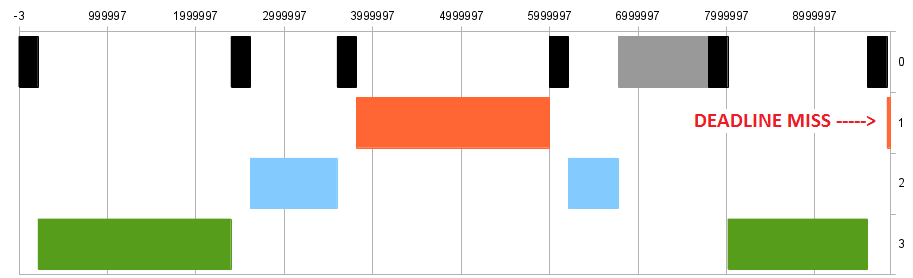
\includegraphics[width=85mm,height=25mm]{images/good/edited/taskset1MeasScenario1.png}
  \caption{ Scenario 1 runtime measured timing diagram}
  \label{scenario1Measurements}
\end{figure}
\end{center}

As shown on the offline timing diagram given in figure \ref{scenario1costs} where the preemption and scheduler costs are taken into account, $t_1$ does not miss its deadline because the scheduler cost is added to the WCET of task $t_1$ during the schedulability analysis, whereas it misses its deadline in the runtime measured timing diagram shown in figure \ref{scenario1Measurements}. 

\begin{center}
\begin{figure}[h]
  \includegraphics[width=85mm,height=25mm]{images/good/edited/taskset1SchedPreemptZoom.png}
  \caption{ Scenario 1 offline timing diagram with scheduler and preemption costs}
  \label{scenario1costs}
\end{figure}
\end{center}

$\bullet$ {\em Second scenario low priority task deadline miss:} here we zoom on the last part of figure \ref{taskSet1Sched}, shown in figure \ref{taskSet1SchedZoom}. When $t_3$ completes its instance, there is still available time before $t_1$ is released. However, since $t_3$ is preempted five times, it pays five preemption and one scheduler costs. When these costs are neglected and are sufficiently large a deadline miss occurs as it is depicted in the runtime measured timing diagram \ref{scenario2Measurements}. 


\begin{center}
\begin{figure}[h]
% \includegraphics[scale=0.3]{images/good/taskset2Sched_scenario2.png}
\includegraphics[width=85mm,height=25mm]{images/good/taskset1Zoom.png}
  \caption{ Task set 1 offline timing diagram}
\label{taskSet1SchedZoom}
\end{figure}
\end{center}


\begin{center}
\begin{figure}[h]
% \includegraphics[scale=0.3]{images/good/taskset2Sched_scenario2.png}
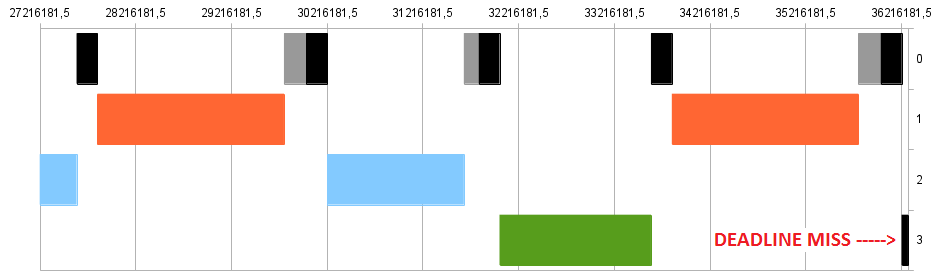
\includegraphics[width=85mm,height=25mm]{images/good/edited/taskset1MeasScenario2.png}
  \caption{ Scenario 2 runtime measured timing diagram}
\label{scenario2Measurements}
\end{figure}
\end{center}


As shown on the zoomed offline timing diagram given in figure \ref{scenario2CostsZoom} where the preemption and scheduler costs are taken into account, $t_3$ misses its deadline, and the utilization factor is greater than one. Consequently, the task set is a priori not schedulable.


\begin{center}
\begin{figure}[h]
% \includegraphics[scale=0.3]{images/good/taskset2Sched_scenario2.png}
\includegraphics[width=85mm,height=25mm]{images/good/taskset1ZoomPreemption.png}
  \caption{ Scenario 2 zoomed offline timing diagram with scheduler and preemption costs}
\label{scenario2CostsZoom}
\end{figure}
\end{center}

The complete offline timing diagram with preemption and scheduler costs is shown in figure \ref{scenario2costs}.




\begin{center}
\begin{figure}[h]
% \includegraphics[scale=0.3]{images/good/taskset2Sched_scenario2.png}
\includegraphics[width=85mm,height=25mm]{images/good/taskset1SchedScenario2.png}
  \caption{ Scenario 2 offline timing diagram with scheduler and preemption costs}
\label{scenario2costs}
\end{figure}
\end{center}



%%%%%%%%%%%%%%%%%%%%%%%%%%%%%%%%

%%%%%%%%%%%%%%%%%%%%%%%%%%%%%%%
%$WCET$ but the preemption and scheduler cost is too big to be contained in this empty space and, therefor because of a %full utilisation factor will cause a deadline miss of the task3 at the very end of scheduling



%%%%%%%%%%%%%%%%%%%%%%%%%%%%%%%GOOD%%%%%%%%%%%
%%%%%%%%%%%%%%%%%%%%%%%%%%%%%%%%%%%%%%%%%%%%%%
%%%%%%%%%%%%%%%%%%%%%%%%%%%%%%%%%%%%%%%%%%%%%%
%%%%%%%%%%%%%%%%%%%%%%%%%%%%%%%%%%%%%%%%%%%%%%
%%%%%%%%%%%%%%%%%%%%%%%%%%%%%%%%%%%%%%%%%%%%%%
%%%%%%%%%%%%%%%%%%%%%%%%%%%%%%%%%%%%%%%%%%%%%%

\subsubsection{Second task set}

the task set described in the table \ref{taskSet2Table} and in the data dependence graph shown in figure \ref{taskSet2DepGraph}, contains three dependent tasks $t_1$, $t_2$ and $t_3$ and one independent task $t_4$. It was scheduled during the offline analysis with an RM algorithm. The corresponding timing diagram is given in figure \ref{taskSet2Sched}. Because of its greatest period, $t_4$ is the lowest priority task. The release dates of higher priority tasks are offseted to avoid mutual preemption, but they have to pay the cost for storing the context of the only preempted $t_4$ and the cost of the scheduler at each release date. Due to this configuration (higher priority tasks are more frequently released than the low priority task $t_4$) several preemptions occurs for one instance of $t_4$. Such situation occurs when for instance a background task is frequently preempeted by  sensor, actuator, and control tasks. The utilization factor of this task set $U=0.7467$ is lower than the utilization factor of the first task set.  



\begin{table}
\caption{Second task set}
\label{taskSet2Table}
\begin{center}
\begin{tabular}{|c|c|c|c|c|}
\hline
\textbf{Tasks} & \textbf{$r_i^1$} & \textbf{$C_i$} & \textbf{$D_i$} & \textbf{$T_i$}  \\
\hline
$t_1$& 30 & 50 & 250  & 250\\
\hline
$t_2$& 120 & 75 & 250  & 250\\
\hline
$t_3$& 200  & 20 & 250  & 250\\
\hline
$t_4$& 0  & 500 & 3000  & 3000\\
\hline
\end{tabular}
\end{center}
\end{table}


\begin{figure}[h]
\begin{center}    
	\includegraphics[scale=1]{images/taskSet2DepGraph.pdf}
	\caption{\label{taskSet2DepGraph} Task set 2 data dependence graph}
 \end{center}   
\end{figure} 


\begin{center}
\begin{figure}[h]
% \includegraphics[scale=0.3]{images/good/taskset2Sched_scenario2.png}
\includegraphics[width=85mm,height=25mm]{images/good/taskset2Sched.png}
  \caption{ Task set 2 offline timing diagram}
\label{taskSet2Sched}
\end{figure}
\end{center}

%here we focus on the last part of figure \ref{taskSet1Sched}, shown at figure \ref{taskSet1SchedZoom}. When $t_3$ %completes its instance, there is still available time before $t_1$ releases. However, since $t_3$ is preempted five %times, and pay one scheduler cost. When these costs are neglected and are sufficiently large a deadline misse occurs as %it is depicted in the runtime measured timing diagram \ref{scenario2Measurements}. 



$\bullet$ {\em Third scenario where preemptions produce other preemptions:} in this scenario we show that when several preemptions occur during one instance of the low priority task $t_4$, these preemptions costs can sufficiently delay the task and cause additional preemptions in a cascading effect, resulting in a deadline miss.  
Here the task $t_4$ is preempted fifteen times according to the offline schedulability analysis shown in the timing diagram given in figure \ref{taskSet2Sched}. Thus, it pays a large value $CP$ that causes the task execution to continue beyond its offline completion time at instant $1230$ pointed by the circle in the zoomed offline timing diagram given in figure \ref{taskSet2SchedZoom}, and pointed at position \textcircled{1} on the zoomed measured timing diagram in figure \ref{scenario3MeasZoom}. Moreover, the task $t_4$ proceeds untill $r_1^6=1280$ the sixth release time of the higher priority task $t_1$. This causes a new preemption for $t_4$ shown at position \textcircled{2} in the zoomed measured timing diagram \ref{scenario3MeasZoom}, and because there is no scheduling table entry afterwards to resume from this additional preemption, as shown after position \textcircled{3} in the zoomed measured timing diagram \ref{scenario3MeasZoom}, $t_4$ misses its deadline. In this case the runtime utilization factor $UE=0.7733$ is not very close to one. However, a deadline miss occurs because of a lack in the scheduling table of the $t_4$ resume entry, corresponding to this additional preemption.       


\begin{center}
\begin{figure}[!h]
% \includegraphics[scale=0.3]{images/good/taskset2Sched_scenario2.png}
\includegraphics[width=85mm,height=25mm]{images/good/taskset2SchedZoom.png}
  \caption{ Task set 2 zoomed offline timing diagram}
\label{taskSet2SchedZoom}
\end{figure}
\end{center}



\begin{center}
\begin{figure}[!h]
% \includegraphics[scale=0.3]{images/good/taskset2Sched_scenario2.png}
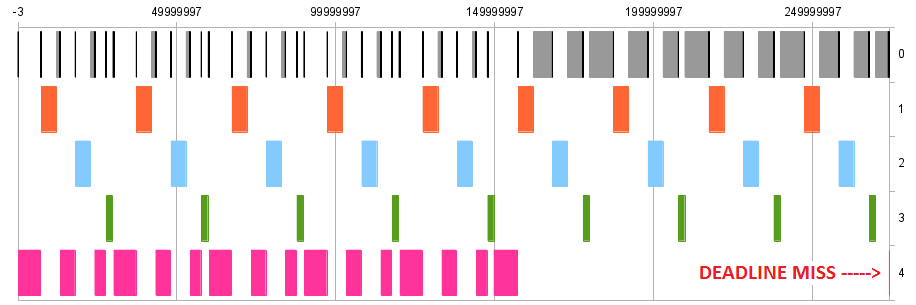
\includegraphics[width=85mm,height=25mm]{images/good/edited/taskset2MeasScenario3.png}
  \caption{ Scenario 3 runtime measured timing diagram}
\label{scenario3Meas}
\end{figure}
\end{center}




\begin{center}
\begin{figure}[!h]
% \includegraphics[scale=0.3]{images/good/taskset2Sched_scenario2.png}
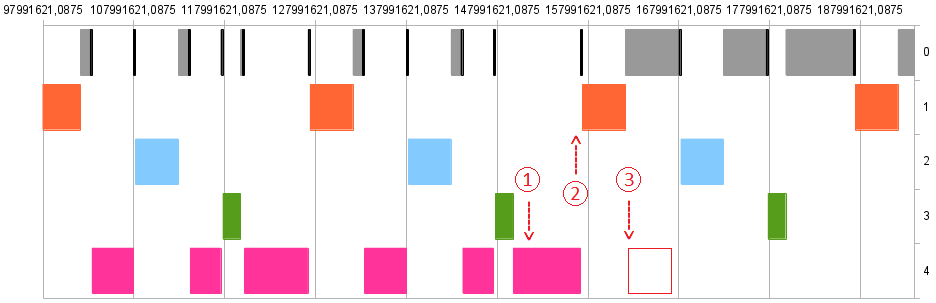
\includegraphics[width=85mm,height=25mm]{images/good/edited/taskset2MeasScenario3Zoom.png}
  \caption{ Scenario 3 zoomed runtime measured timing diagram}
\label{scenario3MeasZoom}
\end{figure}
\end{center}

As shown on the offline timing diagram given in figure \ref{taskSet2SchedZoom} where the preemption and scheduler costs are taken into account, $t_4$ does not miss its deadline, whereas it misses its deadline in the runtime measured timing diagram shown in figure \ref{scenario3MeasZoom}. 



\begin{center}
\begin{figure}[!h]
% \includegraphics[scale=0.3]{images/good/taskset2Sched_scenario2.png}
\includegraphics[width=85mm,height=25mm]{images/good/taskset2SchedScenario3Zoom.png}
  \caption{ Task set 2 offline timing diagram with scheduler and preemption costs}
\label{taskSet2SchedZoom}
\end{figure}
\end{center}

%\subsection{Discussion}
%not taking into account leads to deadline miss 
%taking account:
%deadline miss and not schedulable task set predicted as in scenario two 
%no deadline miss as in scenario 1 and 3

With the proposed approach, we avoid three different deadline miss scenarios by introducing in the schedulability analysis preemptions and scheduler costs. We use a methodology composed of three steps. In the first step we compute the scheduling with an usual offline schedulability analysis that neglects the preemption and scheduler costs. Then in the second step we compare these results with the scheduling measured by running the task set on the Cortex-M4 processor, and we    
observe deadline misses. Finally, we show that the improved offline schedulability analysis taking into account preemption and scheduler costs, avoid deadline misses of scenario one and three, and predicts the deadline miss of scenario two. 


%these scheduling tables are used in a time triggered
%offline scheduler to run the task sets on the Cortex-M4
%processor of the LPC4088 microcontroller. This scheduler
%written in C and assembly implements the algorithm 2.
%Then, we consider three different deadline miss scenarios.
%These experiments show the limitation of this schedulability
%analysis that neglects preemption and scheduler costs. Fi-
%nally, we propose for each scenario, an offline schedulability
%analysis improved by taking into account the preemption and
%scheduler costs.


\section{Conclusion and Future Work}

We proposed a schedulability analysis for data dependent periodic tasks which
precisely accounts for preemption and scheduler costs. The scheduling table
produced by this analysis is exploited in a time triggered offline scheduler
which is perfectly suited for time critical embedded systems, since it
guarantees that no deadline misses occur in accordance with the schedulability
analysis. We evaluated this scheduler on an ARM Cortex-M4 bare metal
processor, and showed that it is able to schedule correctly set of tasks that
miss their deadline when preemption and scheduler costs are neglected.

As future work we plan to extend the present approach to real-time
multiprocessor scheduling. We plan also to take into account more complex
processor architectures including caches which involve CRPD (cache-related
preemption delay) costs that are more complex to master.


\bibliographystyle{unsrt} 
\bibliography{/home/ROCQ/aosteroc/sorel/latex/biblio/bibAutres,/home/ROCQ/aosteroc/sorel/latex/biblio/bibRelatedWork,/home/ROCQ/aosteroc/sorel/latex/biblio/bibSyndex} 
\nocite{}

\end{document}
